\documentclass{article}

\usepackage{amsmath,amssymb,amsthm,graphicx}
\DeclareMathOperator{\disc}{disc}
\DeclareMathOperator{\GL}{GL}
\DeclareMathOperator{\tr}{tr}
\newcommand{\bF}{\mathbf{F}}
\newcommand{\bQ}{\mathbf{Q}}
\newcommand{\bZ}{\mathbf{Z}}
\newcommand{\dd}{\mathrm{d}}
\newcommand{\fr}{\mathrm{fr}}
\newcommand{\Leb}{\mathrm{Leb}}

\newtheorem{corollary}{Corollary}
\newtheorem{conjecture}{Conjecture}

\title{A counterexample relating exponential sums and discrepancy}
\author{Daniel Miller}

\begin{document}
\maketitle





For a prime $p$, let 
\begin{align*}
	T_p &= \left\{ \frac{a}{2\sqrt p} : a\in \bZ, |a|\leqslant 2\sqrt p\right\} \\
	\Theta_p &= \cos^{-1}\left(T_p \right) .
\end{align*}
Since applying continuous increasing functions preserves discrepancy, we have:
\begin{align*}
	\disc(T_p,\Leb) &\ll p^{-1/2} \\
	\disc\left(\Theta_p, \frac 1 2 \sin(t)\, \dd t\right) &\ll p^{-1/2} .
\end{align*}
We claim that starting with $\theta_2\in \Theta_2$, we can choose 
$\theta_p$ such that we preserve the inequalities:
\begin{align*}
	\frac{1}{4\log x} \leqslant \disc(\{\theta_p\}_{p\leqslant x}) \leqslant \frac{4}{\log x} \\
	\left| \sum_{p\leqslant x} U_1(\theta_p)\right| \leqslant 2 \sqrt{x}
\end{align*}
Recall that 
\[
	U_1(\theta) = \frac{\sin(2\theta)}{\sin\theta} .
\]
We can run this for all $p\leqslant {10}^{5}$. Recall that 
$\pi(10^5) \approx 10000$. 

Here is what we get:
\begin{figure}[ht]
\caption{Plot of $\sum_{p\leqslant x} U_1(\theta_p)$}
\centering
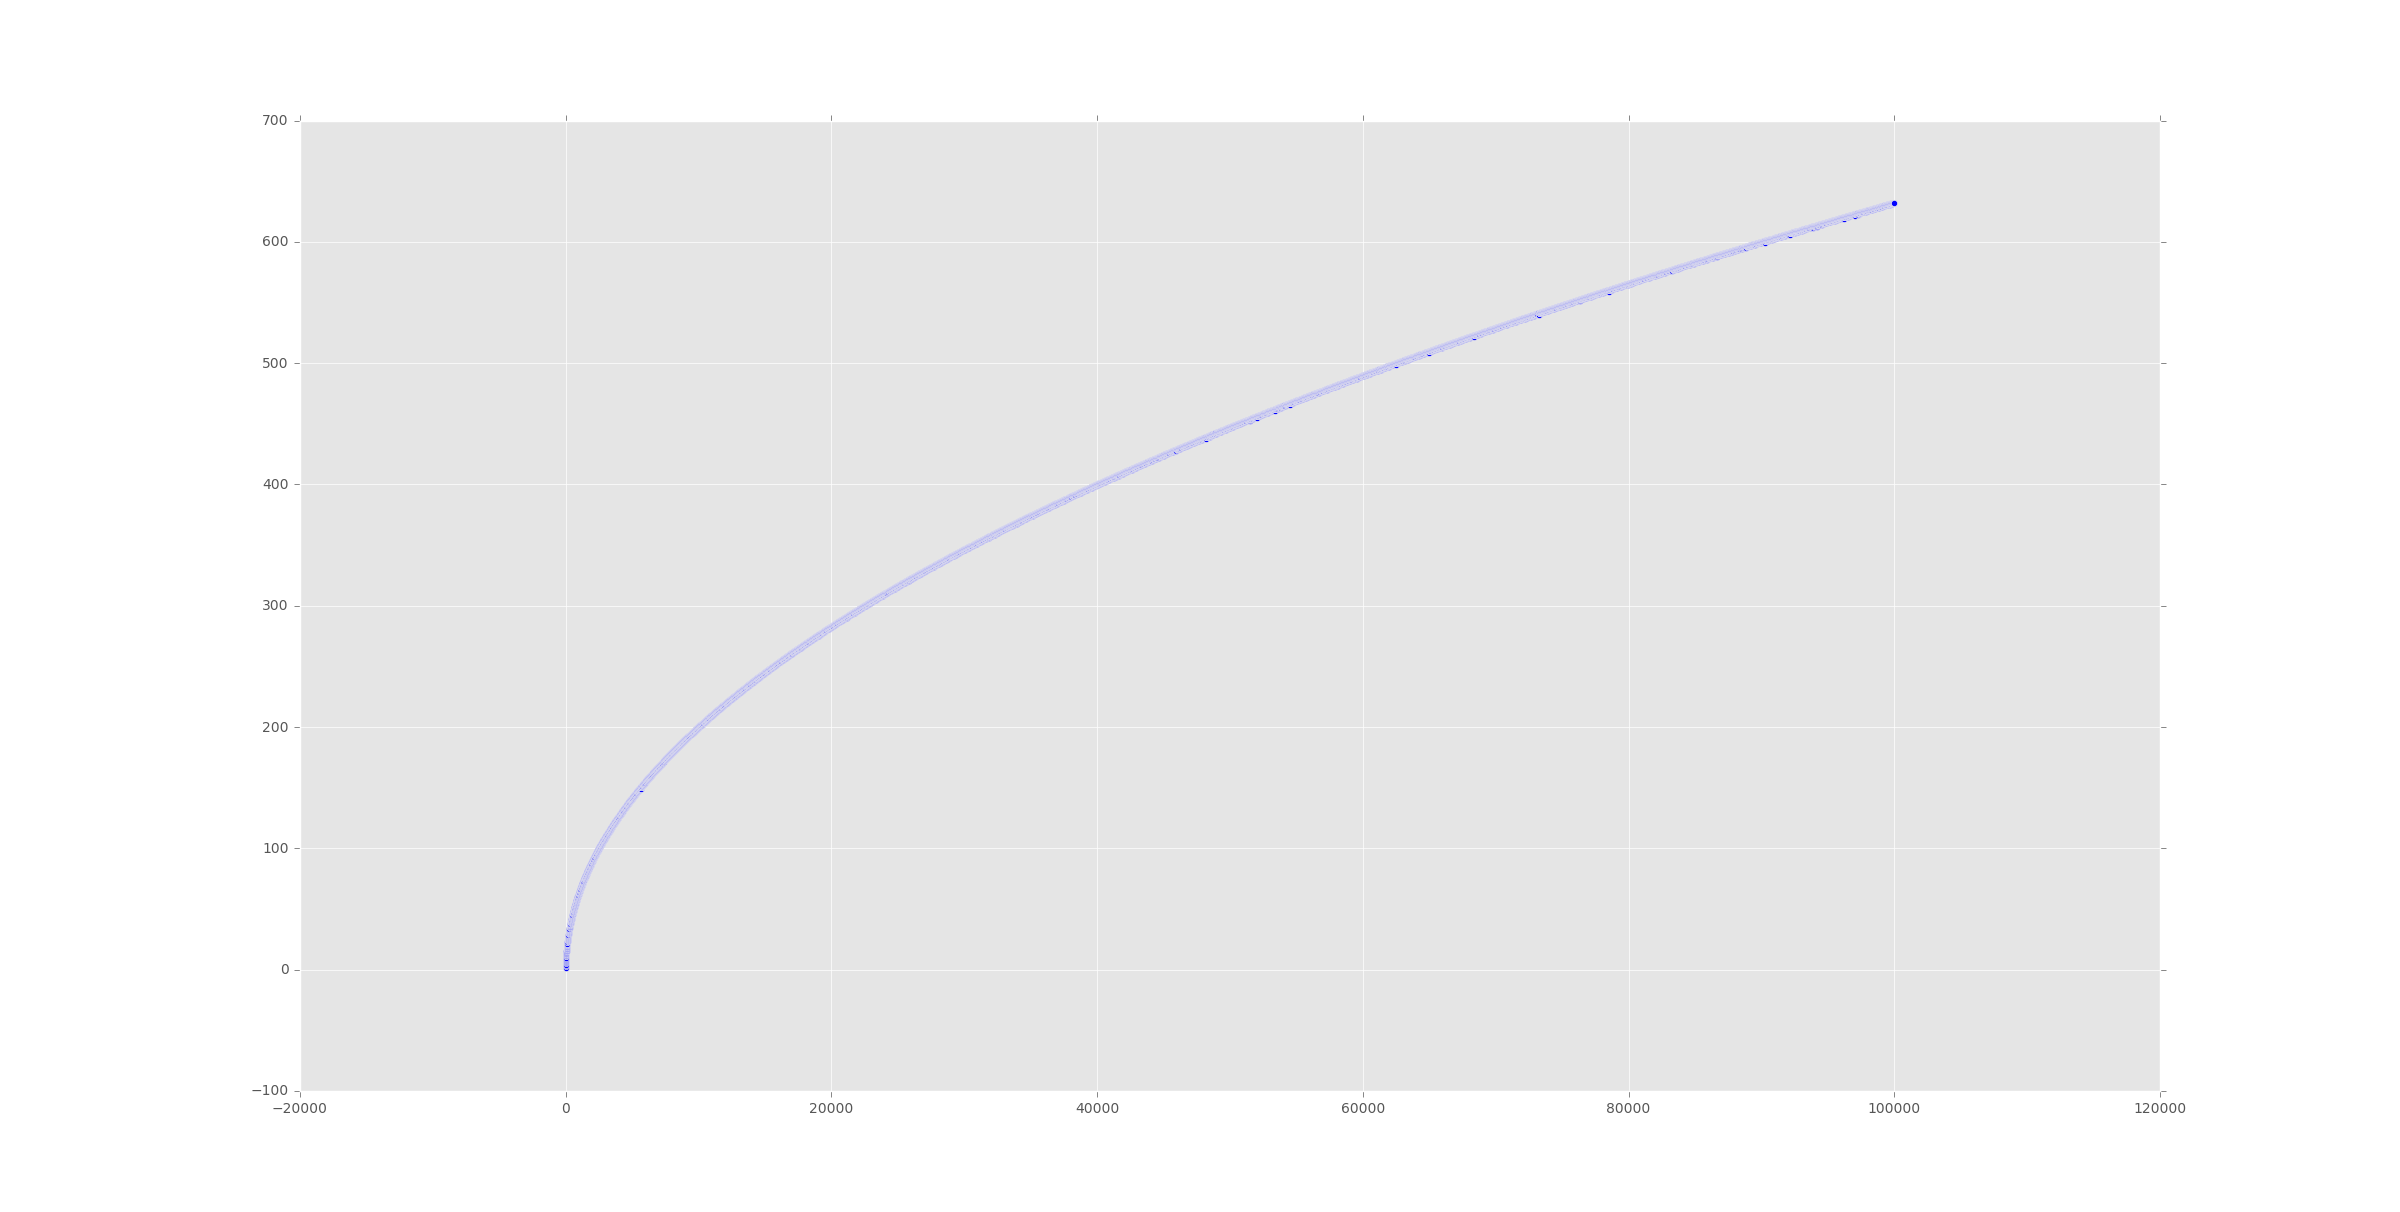
\includegraphics[width=0.8\textwidth]{sums_abs}
\end{figure}

\begin{figure}[ht]
\caption{Plot of $\disc(\{\theta_p\}_{p\leqslant x})$}
\centering
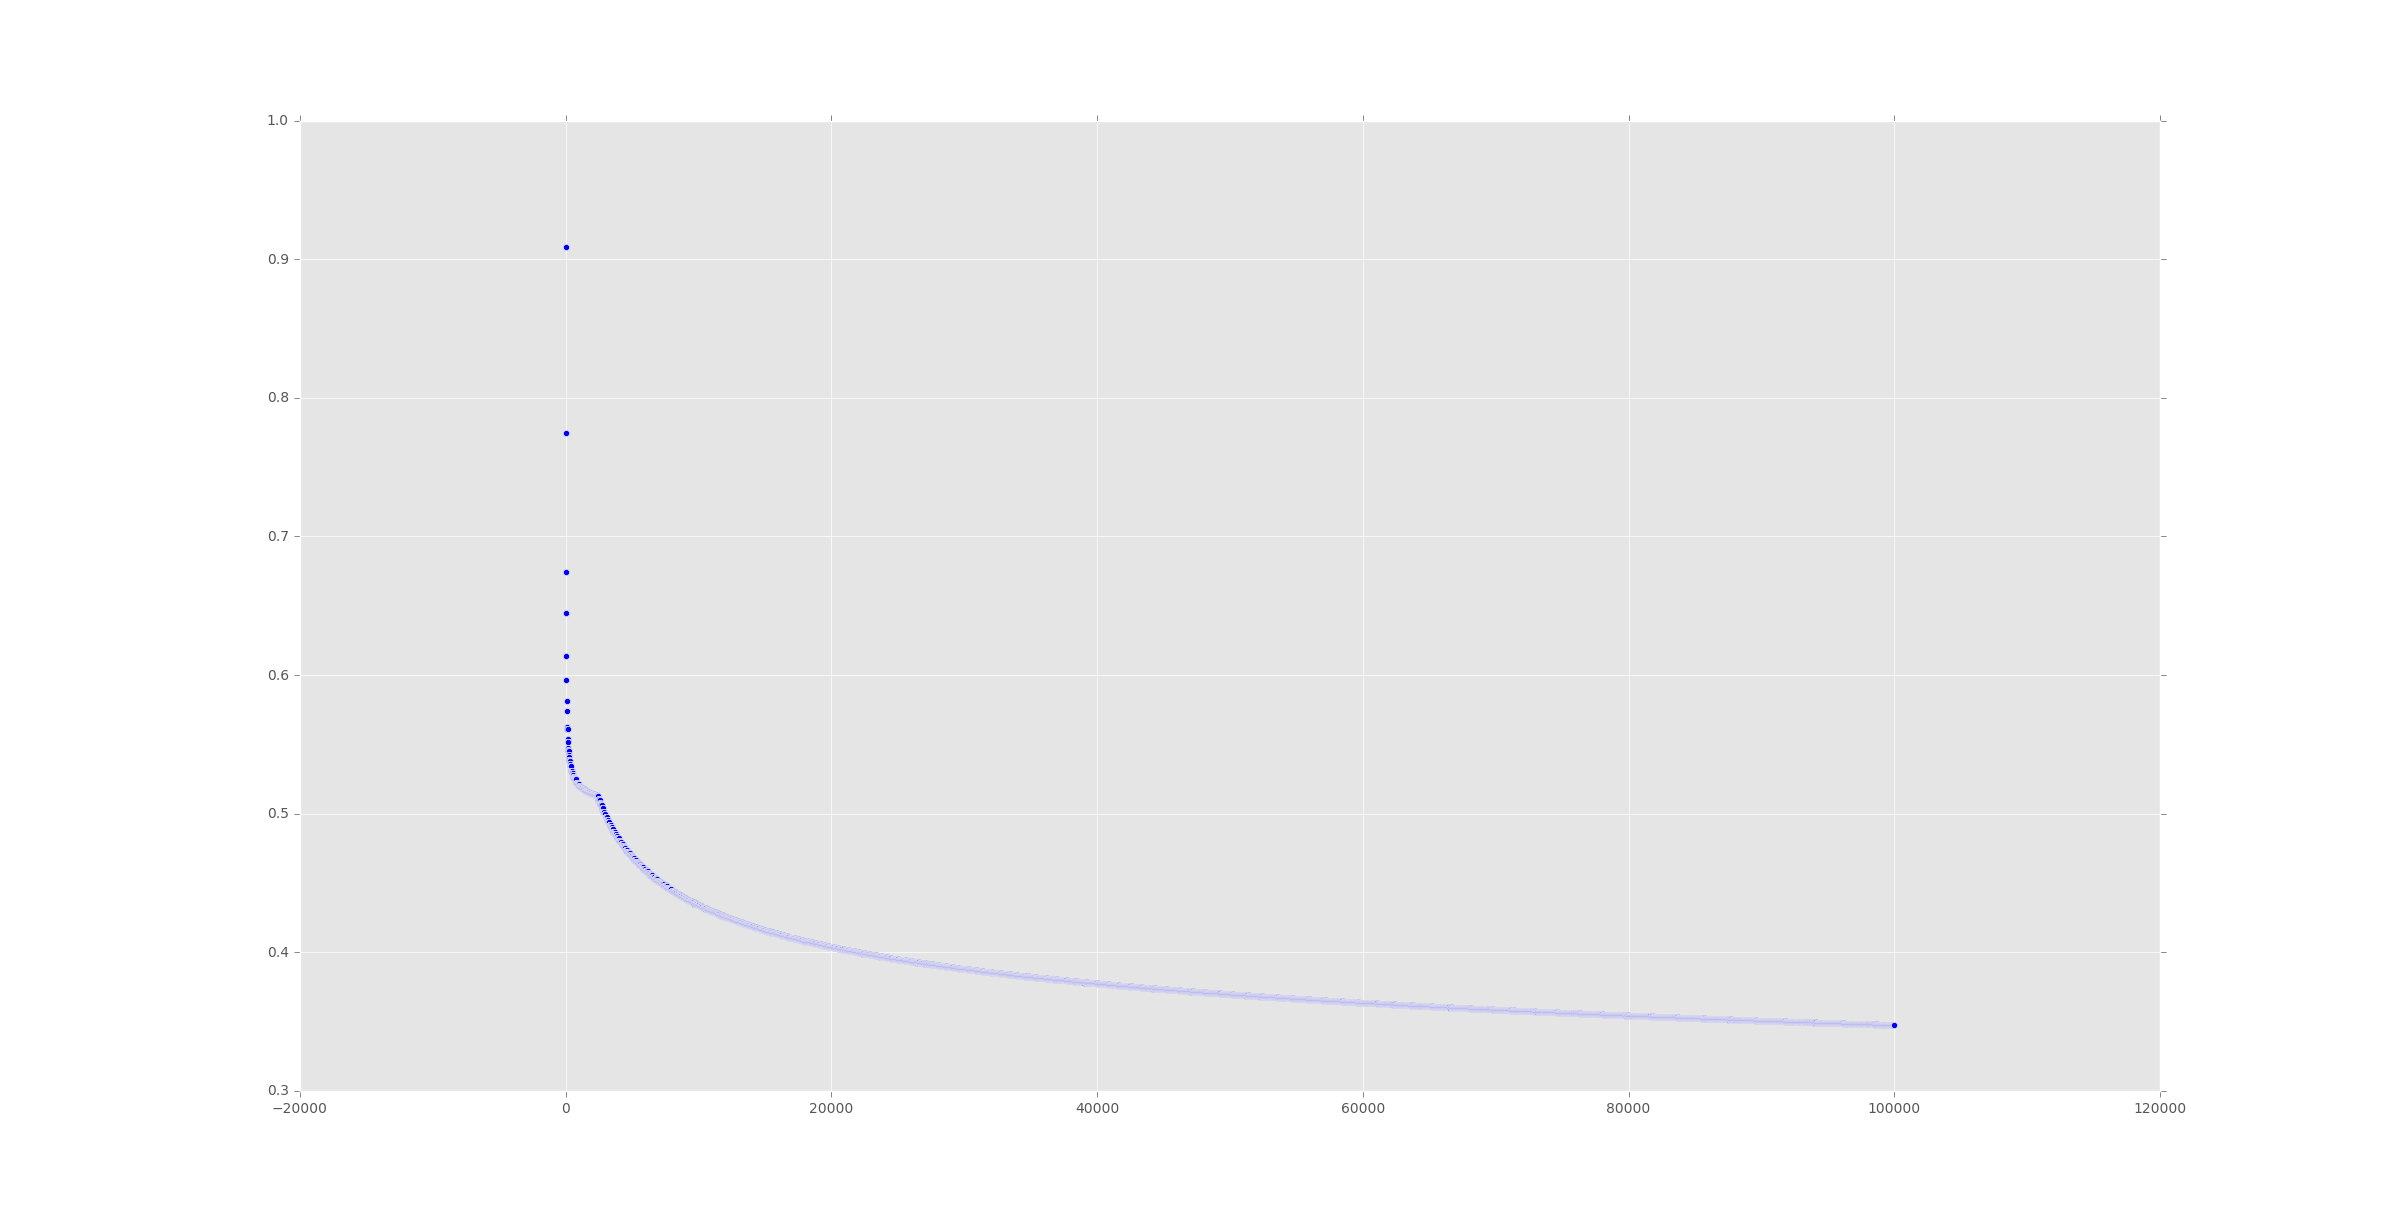
\includegraphics[width=0.8\textwidth]{ks_data}
\end{figure}

\begin{conjecture}
There exists a sequence of $\theta_p\in \Theta_p$ such that the following 
identities always hold:
\begin{align*}
	\frac{1}{4\log x} \leqslant \disc(\{\theta_p\}_{p\leqslant x}) \leqslant \frac{4}{\log x} \\
	\left| \sum_{p\leqslant x} U_1(\theta_p)\right| \leqslant 2 \sqrt{x} .
\end{align*}
\end{conjecture}

Next, choose $\bar\rho_l \colon G_\bQ \twoheadrightarrow \GL_2(\bF_l)$ to 
which we can apply Ramakrishna et.~al.'s machinery. Define 
\[
	\Theta_p(\bar\rho_l) = \left\{\cos\left(\frac{a}{2\sqrt p}\right) : a\in \bZ, |a|\leqslant 2\sqrt p, a \equiv \tr \bar\rho_l(\fr_p)\pmod l\right\} .
\]
\begin{conjecture}
There exists a sequence of $\theta_p\in \Theta_p(\bar\rho_l)$ such that 
\begin{align*}
	\disc(\{\theta_p\}_{p\leqslant x}) =\Omega\left( \frac{1}{\log x} \right)\\
	\left| \sum_{p\leqslant x} U_1(\theta_p)\right| \ll \sqrt{x} .
\end{align*}
\end{conjecture}

\begin{corollary}
There exists an (infinitely ramified) Galois representation 
$\rho_l\colon G_\bQ \to \GL_2(\bZ_l)$ such that if we set 
$a_p = \tr\rho_l(\fr_p)$, then 
\begin{enumerate}
\item
$a_p\in \bZ$
\item
$|a_p| \leqslant 2\sqrt p$ .
\item
The $\theta_p = \cos^{-1}\left(\frac{a_p}{2\sqrt p}\right)$ satisfy 
\begin{align*}
	\disc(\{\theta_p\}_{p\leqslant x}) =\Omega\left( \frac{1}{\log x} \right)\\
	\left| \sum_{p\leqslant x} U_1(\theta_p)\right| \ll \sqrt{x} .
\end{align*}
and hence $L(\rho_l,s)$ satisfies the Riemann Hypothesis. 
\end{enumerate}
\end{corollary}





\end{document}
